\documentclass[../../main.tex]{subfiles}

\begin{document}

\section{Introduction}

In this paper, we examine tunnelling solutions to the 
fundamental equation in quantum mechanics: the Schr\"odinger equation
for a single particle.
\begin{equation}
		\label{eq:schrodinger}
		i \hbar \pder{\Psi}{t} = -\frac{\hbar^2}{2m} \nabla^2 \Psi + 
		V \Psi
\end{equation}
Here $\Psi = \Psi(\vec x)$ is the wave function describing a 
quantum mechanical particle, $t$ is time, 
$V = V(\vec x, t)$ is the potential with which the particle 
interacts.  The constant $m$ is the mass of the particle,
and $\hbar$ is Planck's constant divided by $2\pi$ 
\cite{griffiths-quantum}.  

We consider the following scenario. 
A single particle is confined to an infinitely long cylinder.
This may be approximated as a two dimensional problem,
applying symmetry along the length of the cylinder.
We suppose the cylinder corresponds to a potential well,
posing a potential barrier at the boundary of the cylinder to
the rest of $\R^2$.  

We suppose further there is a second cylinder in the 
vincinity of the first and parallel to it, with its own potential well.
We ask the question: what is the probability the particle will 
tunnel from the first cylinder to the second?
The situation can be summarized in figure \ref{fig:system-sketch}.

\begin{figure}[h]
		\centering
		\includegraphics[width=0.5\textwidth]{system-sketch.png}
		\caption{Two cylindrical potential wells}
		\label{fig:system-sketch}
\end{figure}

To solve this problem using finite elements, first we must compute the weak 
form, then construct the finite dimensional representation.  
Finally, an initial condition must be specified.  
Then solving the problem is the same as evolving the system
forward in time.  

To introduce notation, let $\Omega_0$ denote the first cylinder and 
$\Omega_1$ denote the second (the one without the particle initially).
We suppose the radius of each is $R$ and the distance between their
centers is $L > 2 R$.

\subsection{Nondimensionalization}

Nondimensionalizing the problem is essential since 
$\hbar \approx 10^{-34} J \cdot s$ in S.I. units.  
Let the spacial scaling be $R$, the radius of each of the 
cylinders.  
This induces a time scaling of 
$\frac{2m R^2}{\hbar}$.  
Finally there is an energy scaling of $V_0$.  
To summarize, 
if $\tilde{\vec x}, \tilde t, \tilde V$ all have units, then
\begin{equation}
		\label{eq:nd}
		\tilde{\vec x} = R \vec x, \quad 
		\tilde t = \frac{2m R^2}{\hbar} t, \quad 
		\tilde V(\tilde{\vec x}) = V_0 V(\vec x)
.\end{equation}
Let $\nu = \frac{2mR^2 V_0}{\hbar^2}$.  
The nondimensionalized problem then reads
\begin{equation}
		\label{eq:schrodinger-nondim}
		i \pder{\Psi}{t} = -\nabla^2 \Psi + \nu V(\vec x) \Psi
.\end{equation}
Here, the form of $V(\vec x)$ is 
\begin{equation}
		\label{eq:potential-nondim}
		V(\vec x) = 
		\begin{cases}
				-1 & \vec x \in \Omega_0 \cup \Omega_1 \\
				0 & \text{otherwise}
		\end{cases}
.\end{equation}

\subsection{Boundary Conditions}

Since we are considering the problem defined on all of 
$\R^2$, the required boundary conditions are 
vanishing at infinity.  That is
\begin{equation}
		\label{eq:boundary-conditions}
		\lim_{|\vec x| \to \infty} \Psi(\vec x, t) = 0, \quad 
		\lim_{|\vec x| \to \infty} |\nabla \Psi(\vec x, t)| = \vec 0
\end{equation}
This corresponds with the physical situation that 
the probability of finding the particle infinitely far 
away from either of the cylinders is zero.

\subsection{Initial Conditions}

Since the Schr\"odinger equation is only a first order equation in time,
only $\Psi(\vec x, 0)$ needs to be specified.  
For this, we consider the initial condition corresponding to 
a particle in its lowest energy state, confined to the first cylinder.  
In this situation, only $\Omega_0$ is present, and the potential reads
\begin{equation}
		\label{eq:potential-one-cylinder}
		V^{(0)}(\vec x) = 
		\begin{cases}
				-1 & \vec x \in \Omega_0 \\
				0 & \text{otherwise}
		\end{cases}
\end{equation}

For a quantum particle, its energy states are determined from 
the spatial component of its equation after separation of variables.
Letting $\Psi(\vec x, t) = \psi(\vec x) T(t)$, then this reads
\[
		i \frac{T'}{T} = \frac{-\nabla^2 \psi + \nu V^{(0)} \psi}{\psi} 
		= \epsilon
.\] 
Here $\epsilon$, the eigenvalue, corresponds to 
the energy level of the quantum state \cite{griffiths-quantum}.
Disregarding the time component,
the initial condition for the above problem
solves
\begin{equation}
		\label{eq:init-cond-requirement}
		-\nabla^2 \Psi(\vec x, 0) + \nu V^{(0)} \Psi(\vec x, 0) = 
		\epsilon \Psi(\vec x, 0)
.\end{equation}
Furthermore, this holds for the smallest possible value of 
$\epsilon$.  
\end{document}
